% structure +
% create index +
% create psi +
% bitmap +
% auxiliary data structures +
% ef +
% decode bv->psi +
% decode psi->sa +
% final structure +
% search sa
% complexity +

Let us move on to the implementation of CSA. As it was mentioned in the literature overview,
it is necessary to construct the index the same way as it was done for a suffix array.
It takes $O(n)$ operations \cite{huo2014practical}.

\textbf{CSA structure}

\begin{lstlisting}[caption=CSA structure]
type Csa struct {
	text            string
	suffixOffsets   []int
	psi             []uint64
	length          int
}
\end{lstlisting}

At the listing 4 before a simplified structure of CSA is shown. It consists of the initial text
(only index is compressed, the text remains in the same condition), index, $\psi$-array and a text length.
Index is build with a function that uses suffix array construction algorithm taken from Go library
\cite{golang2016sa}.

\textbf{$\Psi$-array construction}

In order to construct a $\psi$-array, it is necessary to assume that $\psi[0] = \$$. Then make
a traversal over suffix array and find an index that corresponds to a value in suffix array that is
equal to a current one with addition of 1. Listing 5 shows a pseudocode of the algorithm.

\begin{lstlisting}[caption=CSA construction]
	func ConstructPsi() {
		for i < len {
			if sa[j] = sa[i] + 1 {
				psi[i] = j
			}
		}
	}
\end{lstlisting}

\textbf{Additional data structures}

A bitmap from the Roaring.bitmap package \cite{chambi2016better} is used to store the data.
This bitmap implementation is fast and effective. Also Roaring is used at many products such as
Apache Druid, LinkedIn Pinot, Google Procella etc.

Obtained $\psi$-array is a set of monotonically non-decreasing sequences of numbers.
Elias-Fano algorithm allows one to transfer each of these sequences to a bitvector separately.
The quantity of these sequences is equal to the size of alphabet used in a text \cite{andersensimple}.
A question arises: how is it possible to organize the storage of these bitvectors?

One of the solutions is to use two additional arrays:
the first one to store the offset in a $\psi$-array and the second one to store a symbol
corresponding to the ascending sequence.
In this paper text coding is represented by ASCII-code or a less size code.
Thus the alphabet size is limited by 128 symbols. Therefore the size of additional arrays is not
greater than $2 \cdot m$, where $m$ is the size of the alphabet.
An array with offsets is used for a fast indexing over an array of bitmaps.

Additional data structures fulfillment and offsets calculation are performed during the compression
of each separate monotonically non-decreasing sequnce of indices.
To extract these sequences a peroperty described in Lemma \ref{lemma:1} is used,
A termination in ascending of a $\psi$-array corresponds to a symbol switch.
This way it is possible to index bitmaps and fulfill supporting array with symbols of the alphabet used.

\textbf{Elias-Fano}

Compression using Elias-Fano is performed for each separate sequence.
At the same time a preliminary construction of upper and lower parts of bit representation
of the elements of this sequence is performed. The offset is calculated for the following
fast access to lower bits. During the compression procedure, numbers are written in a bitmap,
where it is possible to index over in a constant time.

In order to get access to an element of the sequence (part of $\psi$-array), it is
necessary to use the $select(i)$ function implemented in a bitmap, taking $O(1)$ time.
To check the correctness of the algorithm a function of getting a whole $\psi$-array
was developed appoaching $select(i)$ in it.

\textbf{Suffix array reconstuction}

There is no necessity to completely decode a $\psi$-array to get the access to
an element of a suffix array $sa[i]$. There is a need for performing a traversal over $\psi$-array
until the last element is not reached. Counting the number of steps until the last element $h(i)$,
an index of a decired element can be found by a simple calculation: $sa[i] = n - h(i)$.
This algorithm takes $O(n)$ operations \cite{andersensimple}.

\textbf{Final CSA structure}

After adding supplementary data structures CSA looks as it is shown at the listing 6

\begin{lstlisting}[caption=CSA structure]
type Csa struct {
	text      string
	bv        []*CompressedText
	seqOffset []int
	seqChar   []byte
	length    int
	alphLen   int
}
\end{lstlisting}

It is necessary to emphasize that now there is no need to store indices and additional $\psi$-array.
Instead of that the data is stored in a compressed way in a sequence of bit vectors.
Apart from that the initial text is still stored in the same representation.

Thus to store compressed index it takes $n \cdot \log |\sigma| + o(n)$, where
$|\sigma|$ is an alphabet size. Binary search over suffix array takes $O(\log n)$ operations.
To get an index from a suffix array from a $\psi$-array it is necessary to perform $O(n)$ operations.
In total $O(n\cdot \log n)$ operations are needed to find an element.

\textbf{CSA testing}

Let us consider the efficiency of CSA at the example of five texts with different contexts.
To start, it is required to estimate array construction time and necessary memory storage size.
Table \ref{table:6} shows data for Amazon Text Corpora.

% csa_len = [879, 782, 684, 586, 498, 391, 293, 196, 98, 49, 10, 5, 2] # amazon
% csa_time = [392.040, 299.721, 225.818, 165.427, 114.660, 73.818, 41.825, 18.803, 4.981,
% 1.431, 0.313, 0.269, 0.256] # amazon
% csa_mem = [2281, 2036, 1816, 1573, 1336, 1082, 817, 561, 309, 163, 45, 26, 17] # amazon

\begin{table}[ht!]
	\centering
	\begin{tabular}{|c|c|c|}
		\hline
		\multicolumn{3}{|c|}{Amazon} \\
		\hline
		Text size, KB & Memory, MB & Time, s\\
		\hline
		879 & 2281 & 392.040\\
		\hline
		782 & 2036 & 299.721\\
		\hline
		684 & 1816 & 225.818\\
		\hline
		586 & 1573 & 165.427\\
		\hline
		489 & 1336 & 114.660\\
		\hline
		391 & 1082 & 73.818\\
		\hline
		293 & 817 & 41.825\\
		\hline
		196 & 561 & 18.803\\
		\hline
		98 & 309 & 4.981\\
		\hline
		49 & 163 & 1.431\\
		\hline
		10 & 45 & 0.313\\
		\hline
		5 & 26 & 0.269\\
		\hline
		2 & 17 & 0.256\\
		\hline
	\end{tabular}
	\caption{CSA construction}
	\label{table:6}
\end{table}

\begin{figure}[ht!]
	\centering
	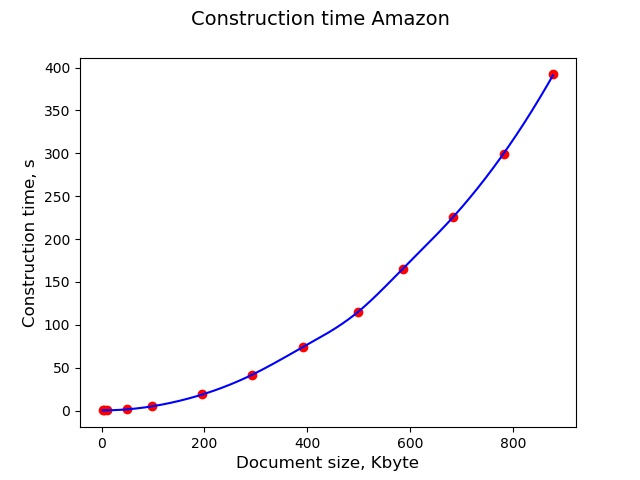
\includegraphics[width=12cm]{construct_time_amazon}
	\caption{CSA construction}
	\label{fig:CSA_construct_time_amazon}
\end{figure}

\begin{figure}[ht!]
	\centering
	\begin{subfigure}[b]{0.49\textwidth}
		\centering
		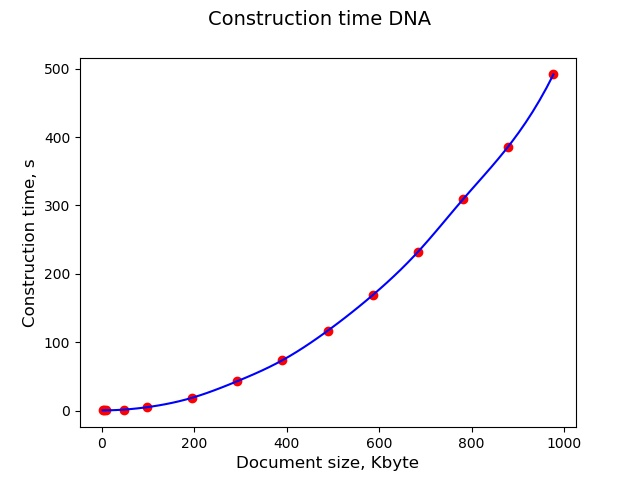
\includegraphics[width=\textwidth]{construct_time_DNA}
		\caption{DNA}
		\label{fig:y equals x}
	\end{subfigure}
	\hfill
	\begin{subfigure}[b]{0.49\textwidth}
		\centering
		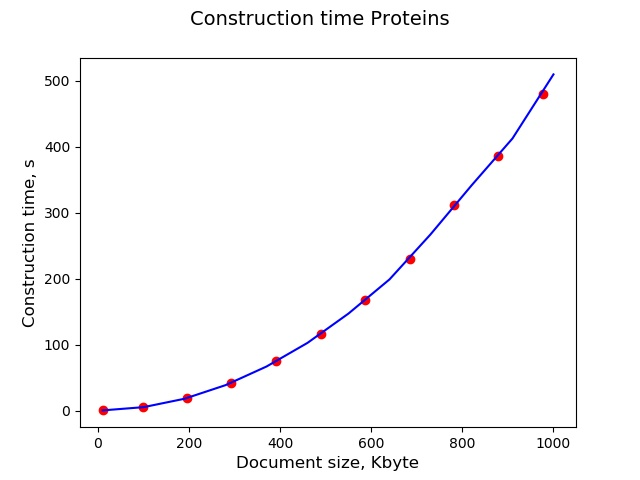
\includegraphics[width=\textwidth]{construct_time_Proteins}
		\caption{Proteins}
		\label{fig:three sin x proteins}
	\end{subfigure}
	\hfill
	\begin{subfigure}[b]{0.49\textwidth}
		\centering
		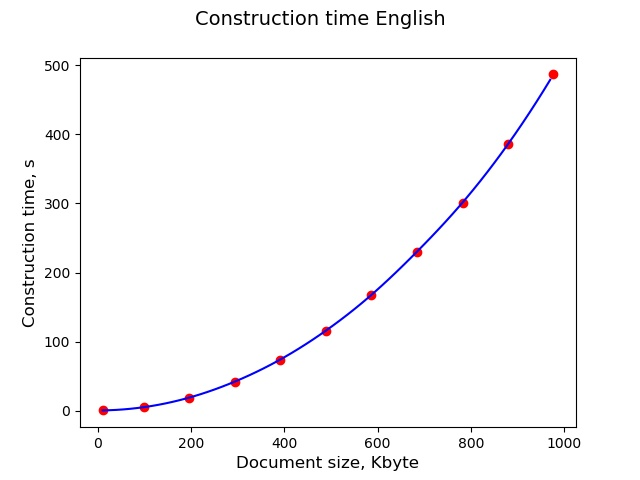
\includegraphics[width=\textwidth]{construct_time_English}
		\caption{English}
		\label{fig:three sin x english}
	\end{subfigure}
	\hfill
	\begin{subfigure}[b]{0.49\textwidth}
		\centering
		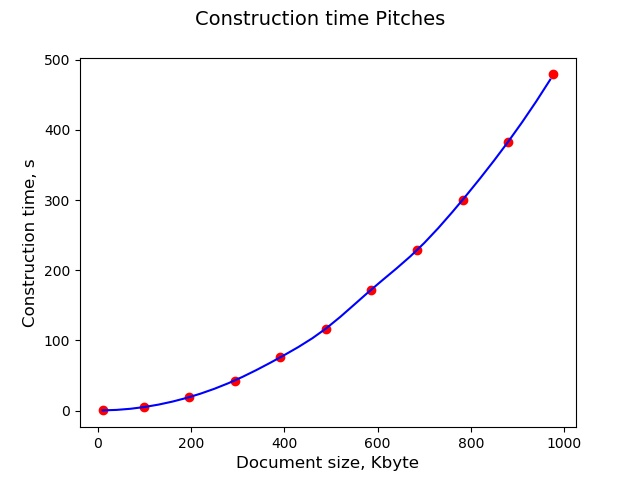
\includegraphics[width=\textwidth]{construct_time_Pitches}
		\caption{Pitches}
		\label{fig:three sin x pitches}
	\end{subfigure}
	\caption{CSA construction}
	\label{fig:three graphs}
\end{figure}

\begin{figure}[ht!]
	\centering
	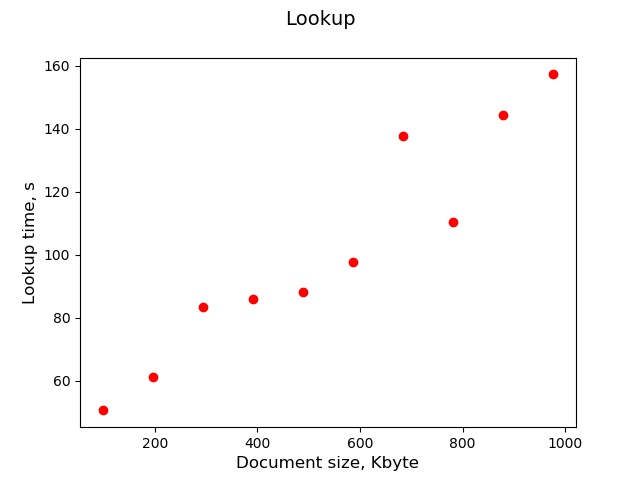
\includegraphics[width=12cm]{Lookup_time_csa_amazon}
	\caption{Substring lookup in CSA}
	\label{fig:CSA_Lookup_time_csa_amazon}
\end{figure}

\clearpage
\newpage

Let us consider the results of a dependency between a substring lookup speed and a text size for CSA,
suffix array and radix tree constructed for Amazon Text Corpora. Figure \ref{fig:CSA_Lookup_time}
shows that a substring lookup speed for a fixed size substring does not depend on the text size for
suffix array and radix tree. Lookup time increases with increasing of the size of the initial text for CSA.
Radix tree shows the best result as it was expected.

\begin{figure}[ht!]
	\centering
	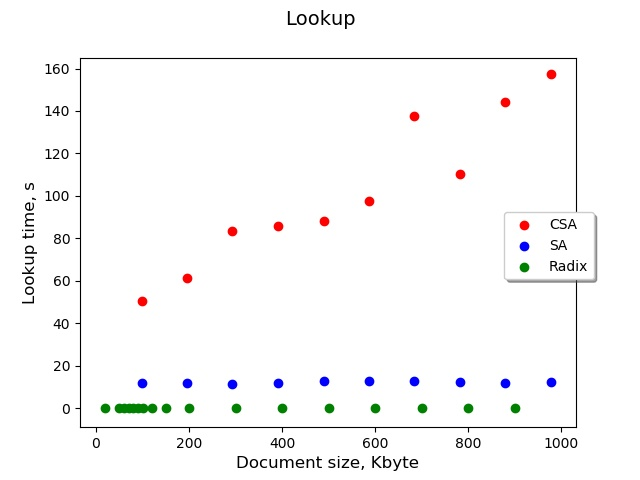
\includegraphics[width=12cm]{Lookup_time}
	\caption{Substring lookup time in CSA}
	\label{fig:CSA_Lookup_time}
\end{figure}
